
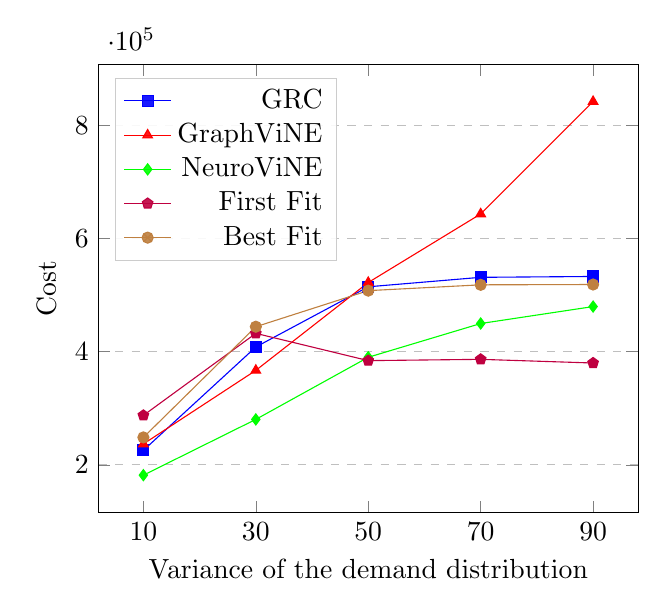
\begin{tikzpicture}
\begin{axis}[
    legend cell align={right},
    legend style={fill opacity=0.9, draw opacity=1, text opacity=1, draw=white!80!black},
    xlabel={Variance of the demand distribution},
    ylabel={Cost},
    % xmin=0, xmax=100,
    % ymin=0, ymax=1,
    xtick={0,10,30,50,70,90, 100},
    % ytick={0,100,200,300,400,500},
    legend pos=north west,
    ymajorgrids=true,
    grid style=dashed,
]

\addplot[
    color=blue,
    mark=square*,
    ]
    coordinates {
(10,225549)
(30,408456)
(50,514992)
(70,531753)
(90,533247)
    };
\addlegendentry{GRC}

\addplot[
    color=red,
    mark=triangle*,
    ]
    coordinates {
(10,236842)
(30,367070)
(50,522564)
(70,643883)
(90,842784)
    };
\addlegendentry{GraphViNE}

\addplot[
    color=green,
    mark=diamond*,
    ]
    coordinates {
(10,181638)
(30,280335)
(50,390260)
(70,449987)
(90,479996)
    };
\addlegendentry{NeuroViNE}

\addplot[
    color=purple,
    mark=pentagon*,
    ]
    coordinates {
(10,287405)
(30,432565)
(50,384316)
(70,386606)
(90,380101)
    };
\addlegendentry{First Fit}

\addplot[
    color=brown,
    mark=otimes*,
    ]
    coordinates {
(10,248473)
(30,444340)
(50,508184)
(70,518467)
(90,519020)
    };
\addlegendentry{Best Fit}





\end{axis}
\end{tikzpicture}